% This is samplepaper.tex, a sample chapter demonstrating the
% LLNCS macro package for Springer Computer Science proceedings;
% Version 2.20 of 2017/10/04
%
\documentclass[runningheads]{llncs}
%
\usepackage{graphicx}
\usepackage{multirow} 
\usepackage{fancyvrb}
\usepackage[misc,geometry]{ifsym} 
\usepackage{subcaption}
\usepackage{caption}
% Used for displaying a sample figure. If possible, figure files should
% be included in EPS format.
%
% If you use the hyperref package, please uncomment the following line
% to display URLs in blue roman font according to Springer's eBook style:
% \renewcommand\UrlFont{\color{blue}\rmfamily}

\begin{document}
%
\title{Formal Grammars and Neural Networks for RNA Secondary Structure Prediction\thanks{Supported by the Russian Science Foundation grant 18-11-00100}}
%
%\titlerunning{Abbreviated paper title}
% If the paper title is too long for the running head, you can set
% an abbreviated paper title here
%
\author{Polina Lunina\inst{1,2}\orcidID{0000-0002-7172-2647} \Letter \and
Semyon Grigorev\inst{1,2}\orcidID{0000-0002-7966-0698}}
%
\authorrunning{Polina Lunina, Semyon Grigorev}
% First names are abbreviated in the running head.
% If there are more than two authors, 'et al.' is used.
%
\institute{Saint Petersburg State University, 7/9 Universitetskaya nab., St. Petersburg, 199034, Russia \and
JetBrains Research, Primorskiy prospekt 68-70, Building 1, St. Petersburg 197374, Russia\\
\email{lunina\_polina@mail.ru \Letter, semyon.grigorev@jetbrains.com, s.v.grigoriev@spbu.ru}\\
}
%
\maketitle             % typeset the header of the contribution
%
\begin{abstract}
RNA secondary structure prediction problem is known to be quite critical in computational genomics, therefore, different tools and algorithms are still competing in this field. In this work, we propose a new approach for secondary structure prediction. We describe the most probable types of stems by a context-free grammar, suchwise, the parsing matrix for some sequence represents all the theoretically possible stems. Then we apply an ensemble of residual neural networks to process such matrices in order to get a contact map of a pure secondary structure. RNA secondary structure databases are not big enough for neural network training, so, we use transfer learning technique. Firstly, we train several base networks with prediction tools output as a reference data, and secondly, we transfer these networks weights to a final composite model, which is trained and evaluated on real world data.

\keywords{CNN \and ResNet \and Machine Learning \and Secondary Structure \and Genomic Sequences \and Formal Grammars \and Parsing.}
\end{abstract}
%
%
%
\section{Introduction}
Improvement in RNA secondary structure prediction accuracy is one of the key focuses in computational genomics due to its crucial role in functional analysis of RNA molecules. All the diversity of existing secondary structure prediction techniques can be divided into comparative methods that analyse several homologous sequences employing evolutionary approaches~\cite{hofacker1999automatic,tahi2002automatic} and single sequence methods that process one sequence at a time according to some folding constraints, e.g. thermodynamic~\cite{hamada2009prediction} or statistic~\cite{eddy1994rna,do2006contrafold} rules. One of the challenging parts is pseudoknotted structures processing, because pseudoknots are known to be widely represented in biological data, including functionally important RNA regions, nevertheless, building a model that handles them has always been a non-trivial task.

Among other ways, formal grammars can be applied for RNA secondary structure description and some of the algorithms utilize this technique for secondary structure prediction~\cite{knudsen2003pfold,nebel2011evaluation}. Due to probabilistic nature of secondary structure formation laws complicated stochastic (probabilistic) grammars are generally used here.

In this work, a new approach to secondary structure prediction which employs the combination of ordinary formal grammars and artificial neural networks is presented. The main ideas were outlined in~\cite{grigorevcomposition,lunina2019secondary} and this research is conducted to further development of this approach in the context of secondary structure prediction problem. Secondary structure can be formally described as a compositions of stems having different lengths and loop sizes~\cite{MQbioinformatics19}, so, we propose to use a simple context-free (not probabilistic) grammar to encode the most common types of stems and search for such stems in the input sequences by matrix-based parsing algorithm. Thereby, the parsing matrix for some sequence will contain the information about whether each subsequence of this sequence can fold to stem or not. This matrix is not yet a representation of a valid secondary structure, because it cannot contain all these stems at once and, besides, there can be more complex elements that are not expressible in terms of our grammar (such as pseudoknots and non-canonical base pairs). Therefore, we propose to process such matrices by neural networks that should filter extra stems and add some missing elements in order to generate a maximal approximation of this sequence secondary structure.

\section{Proposed Approach Overview}
In this section the brief description of the approach proposed in~\cite{grigorevcomposition,lunina2019secondary} is provided. Although these works were devoted to RNA sequences classification problems, the main ideas are still relevant in the context of the current research. The proposed approach combines two different techniques: firstly, we use formal grammars for secondary structure features description and secondly, we apply neural networks for these features processing and building a final solution.

\subsubsection{Formal Grammars}
The classical way of formal languages application for secondary structure description is to model the whole structure by means of probabilistic grammars~\cite{knudsen2003pfold,nebel2011evaluation}. This approach is known to be quite successful, but it also should be mentioned that building such grammar requires a lot of theoretical and practical difficulties. Therefore, we propose a different way --- to encode only stems of secondary structure by simple context-free grammar and leave further processing and probability estimation to neural network. 

In figure~\ref{gram} grammar $G_0$ that we use in this work as well as in the previous ones is presented. This grammar describes the recursive compositions of stems having height at least 3 (lines \textbf{7-12}) and loop size from 2 up to 10 (line \textbf{2}). Note that these constants are not mandatory and might be defined experimentally for each task. Also, $G_0$ allows only conventional base pairs (line \textbf{5}) and does not express pseudoknots, because adding the rules for both of these features complicates the grammar in unacceptable for us way, therefore, we expect the neural network to handle them. Also, we consider only stems of height three or more, because including shorter stems would overload the parsing matrix with unnecessary information. So, a sequence folds to a stem (according to the rules we have just defined) iff it is derivable from start nonterminal $s1$ of $G_0$ (line \textbf{1}).

\begin{figure}[ht]
\begin{Verbatim}[numbers=left,xleftmargin=5mm]
s1: stem<s0>
any_str : any_smb*[2..10]
s0: any_str | any_str stem<s0> s0
any_smb: A | U | C | G
stem1<s>: A s U | G s C | U s A | C s G 
stem2<s>: stem1< stem1<s> >
stem<s>:  
      A stem<s> U 
    | U stem<s> A 
    | C stem<s> G 
    | G stem<s> C 
    | stem1< stem2<s> >  
\end{Verbatim}
\caption{Context-free grammar $G_0$ for RNA secondary structure stems description}
\label{gram}
\end{figure}

Having a grammar, we want to find all the subsequences of some given sequence that may fold to stems and this is to be done by parsing algorithm. In all the experiments we use parsing algorithm~\cite{Azimov:2018:CPQ:3210259.3210264} that is based on matrix operations and demonstrates high performance in practice due to the effective use of GPGPU. 

Formally, the result of a matrix-based parsing algorithm for an input string $w$ is an upper-triangular boolean matrix $M_P$, where $M_P [i,j] = 1$, iff the substring $w[i,j]$ is derivable from grammar start nonterminal. From the practical point of view, this means that parsing matrix contains 1 in a cell iff a correspondent substring folds to a stem according to the rules of a given grammar, so each stem results in a diagonal chain of one-s in the matrix, because if sequence $w_1...w_n$ is a stem than it is clear that $w_2...w_{n - 1}$ is a stem and $w_3...w_{n - 2}$ is a stem and so on while the stem height is at least 3.

In the figure~\ref{pars_res} we provide a parsing result for a short tRNA sequence and show how parsing matrix maps with secondary structure stems. Each 1 in cell describes the stem of height at least 3, so, this sequence contains two subsequences that may fold to stems of the first nesting level. These stems expected hydrogen bonds along with corresponding matrix cells are painted in two different colors. Note that these stems interfere with each other, thereby, real secondary structure cannot contain both of them at the same time.


\begin{figure}
\centering
\valign{#\cr
  \hbox{%
    \begin{subfigure}[b]{.6\textwidth}
    \centering
    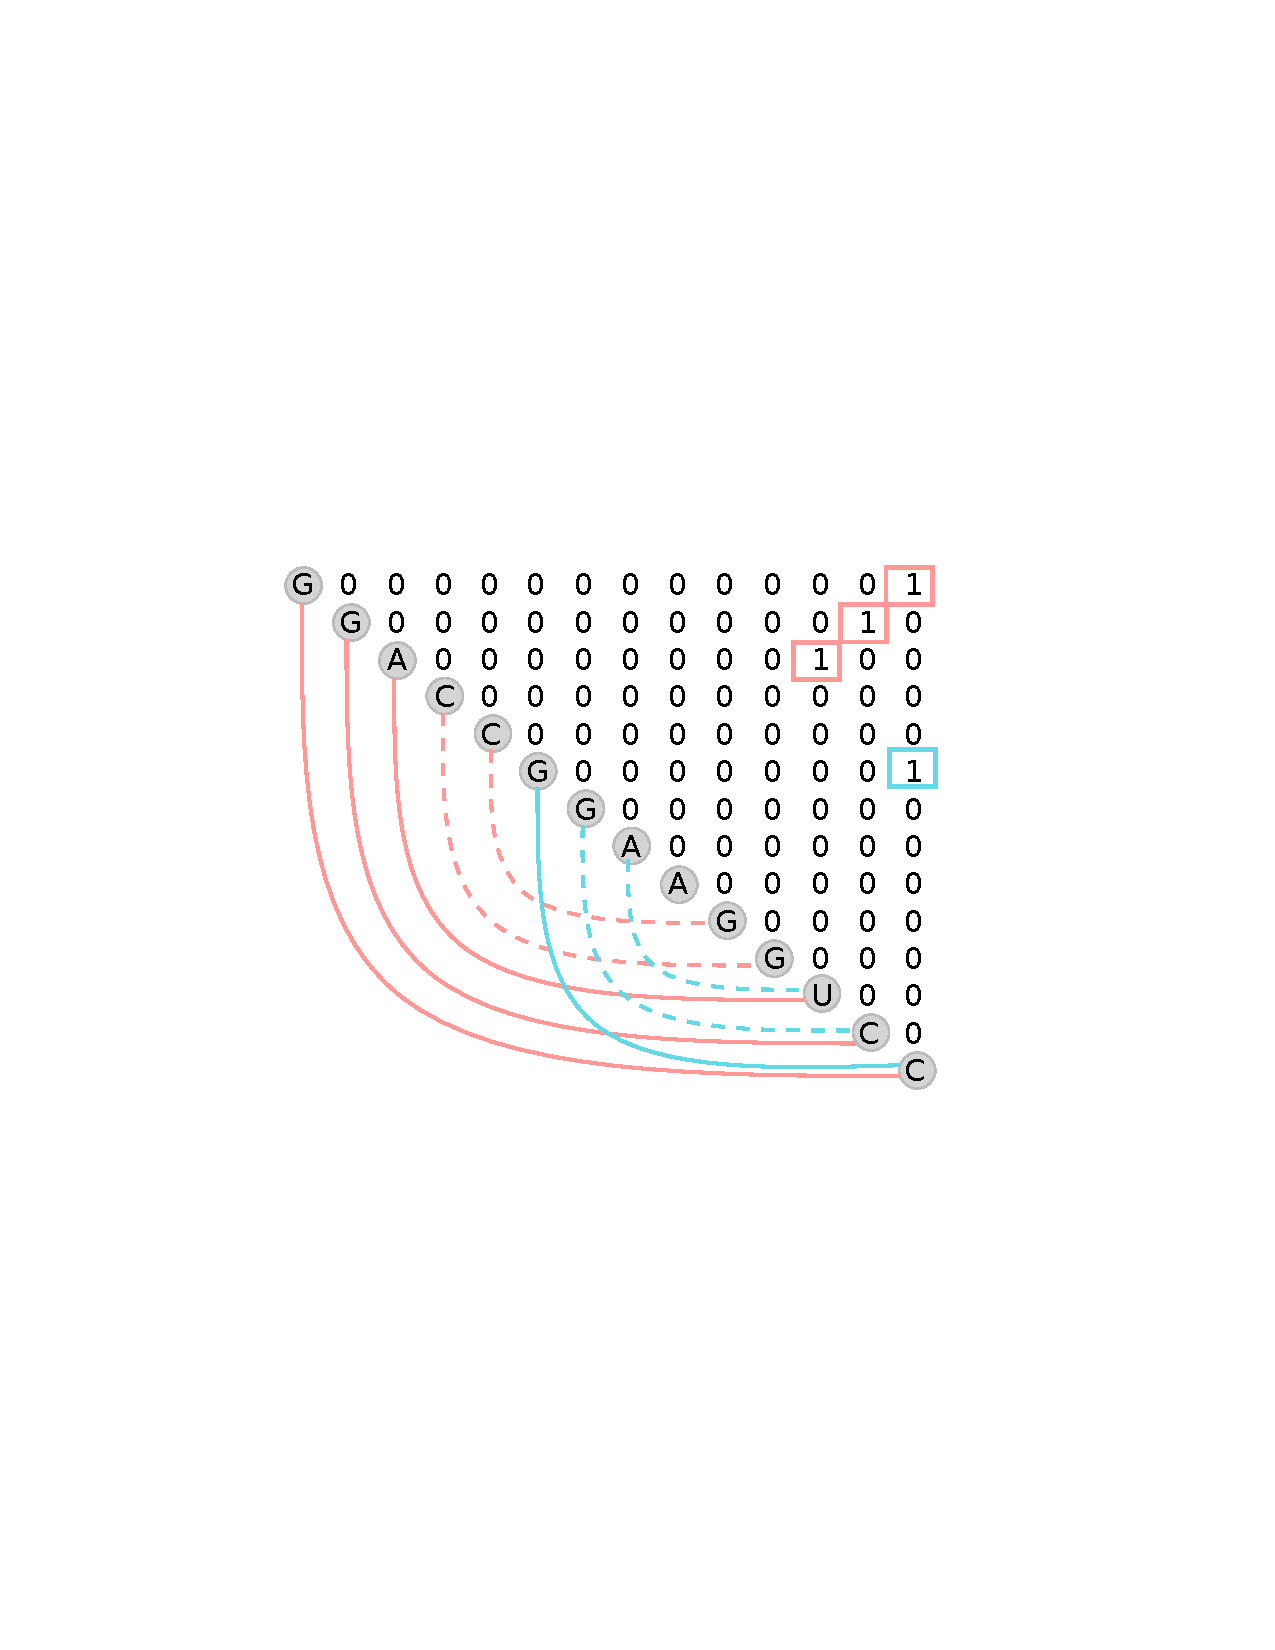
\includegraphics[width=\textwidth]{pics/matrix.pdf}
    \caption{Parsing matrix}
    \label{mtrx}
    \end{subfigure}%
  }\cr
  \noalign{\hfill}
  \hbox{%
    \begin{subfigure}{.4\textwidth}
    \centering
    \vspace{2mm}
    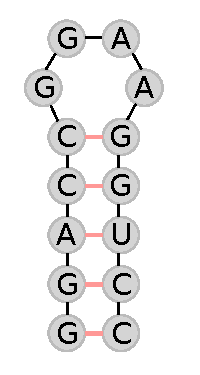
\includegraphics[width=.3\textwidth]{pics/stem1.pdf}
    \caption{First stem}
    \label{stem1}
    \end{subfigure}%
  }\vfill
  \hbox{%
    \begin{subfigure}{.4\textwidth}
    \centering
     \vspace{-2mm}
    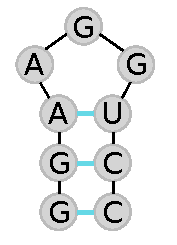
\includegraphics[width=.3\textwidth]{pics/stem2.pdf}
    \caption{Second stem}
    \label{stem2}
    \end{subfigure}%
  }\cr
}
\caption{Stems extracted from tRNA sequence}
\label{pars_res}
\end{figure}


\subsubsection{Neural Networks}
Parsing matrix is yet a formal construction storing the information about secondary structure features, so, at the final step of our solution we propose to use artificial neural networks, to process such matrices and correlate them with some real world data. Matrices should be transformed to any suitable format and sent to the input layer of a neural network, constructed for a specific task. For example, in~\cite{lunina2019secondary} we provide examples of neural networks for small RNA classification problems and show how to process parsing matrices as numerical vectors and black-and-white images.


\subsection{Secondary Structure Prediction}
In this section we describe all the details of the proposed approach application concerning specifically secondary structure prediction task. 
\subsubsection{Motivation}
One of the classical ways of RNA secondary structure formal representation is so-called contact map which for an input string $w$ is a boolean matrix $M_C$, where $M_C [i,j] = 1$, iff nucleotides in positions $i$ and $j$ form a hydrogen bond (or, to put it simply, a contact) in secondary structure. Consider the discussed earlier parsing matrix for the same sequence $w$ that has 1 in the cell $[i, j]$, iff subsequence $w[i, j]$ folds to a stem. It is clear that the first and the last nucleotides of every stem form a contact, therefore, we can easily transfer between parsing matrix and contact map definitions and view the parsing matrix as a sort of a contact map. Note that if parser finds a stem of height three than we will see only one cell with $1$ in matrix, but such stem always wraps a stem of height two which wraps a stem of height one, so, we are always missing two contacts, therefore, after parsing we set $M_P[i - 1, j + 1] := 1$ , $M_P[i - 2, j + 2] := 1$ if $M_P[i][j] = 1$, $i = 0..size(M_p), j = i..size(M_p)$.

In the figure~\ref{struc} we provide two-dimensional secondary structure visualization for tRNA sequence (the plot~\ref{struc_a} was made by tool~\cite{kerpedjiev2015forna}) with corresponding contact and parsing matrices and it can be seen clearly that the actual amount of contacts is far less than parsing matrix contains. Moreover, our grammar has certain limitations and cannot, for example, describe pseudoknots and non-canonical base pairs, so, the contacts that are formed by such rules will not be reflected in the parsing matrix. 

\begin{figure}[h]
\centering
\begin{subfigure}{.3\textwidth}
  \centering
  \fbox{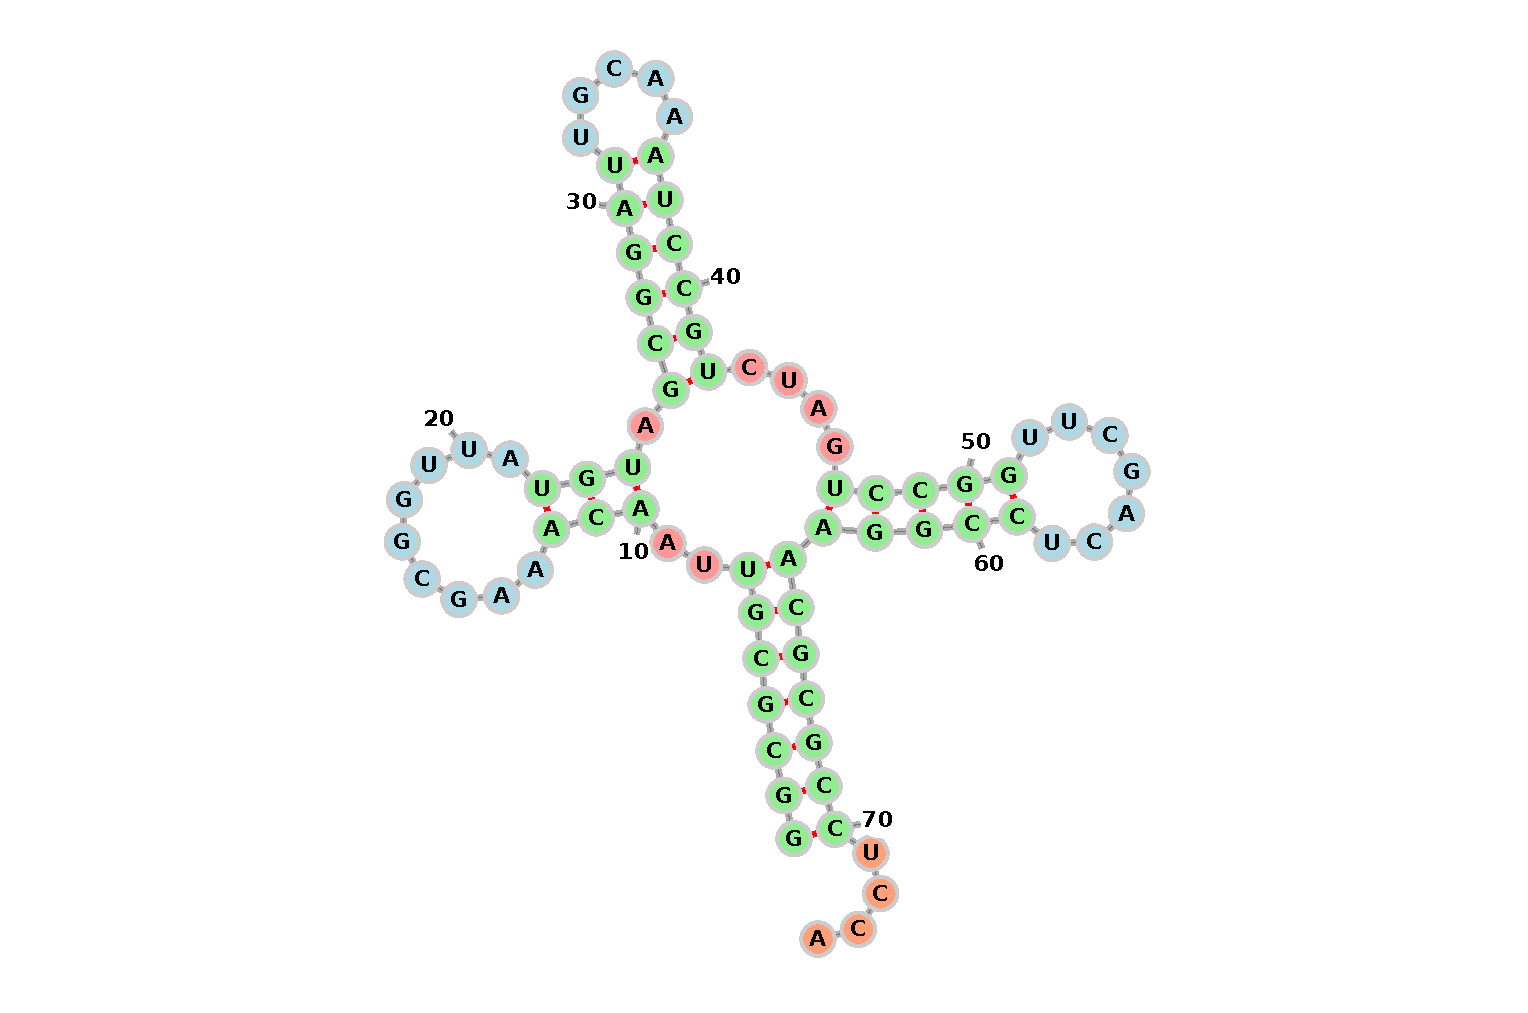
\includegraphics[width=.85\linewidth]{pics/rna.pdf}}
  \caption{Visualization}
  \label{struc_a}
\end{subfigure}%
\begin{subfigure}{.3\textwidth}
  \centering
  \fbox{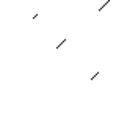
\includegraphics[width=.85\linewidth]{pics/img_ref.pdf}}
  \caption{Contact matrix}
  \label{struc_b}
\end{subfigure}
\begin{subfigure}{.3\textwidth}
  \centering
  \fbox{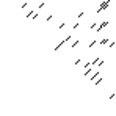
\includegraphics[width=.85\linewidth]{pics/img_pars.pdf}}
  \caption{Parsing matrix}
  \label{struc_c}
\end{subfigure}
\caption{RNA secondary structure representations}
\label{struc}
\end{figure}

So, our task is set as follows: we want to process parsing matrices by a neural network in order to achieve a maximal similarity with the expected sequence secondary structure. This network should take parsing matrices as inputs and contact maps as desired outputs for the same set of RNA sequences. For convenience, we transform both matrices to black-and-white images by replacing zero cells with black pixels and one cells with white pixels. Also, we code sequences at the images diagonals by four types of gray pixels in case the nucleotide chains contain some important information about secondary structure shape.

\subsubsection{Reference data}

\subsubsection{ResNet}

\subsection{Experiments}

%
\bibliography{main} 
\bibliographystyle{ieeetr}
\end{document}
